%!TEX root = /Users/ego/Boulot/TKZ/tkz-euclide/doc_fr/TKZdoc-euclide-main.tex

\section{Les secteurs}

\begin{NewMacroBox}{tkzDrawSector}{\oarg{local options}\parg{O,\dots}\parg{\dots}}
\noindent\emph{Attention les arguments varient en fonction des options.}

\medskip
\begin{tabular}{lll}
\toprule
options             & défaut & définition                         \\ 
\midrule
\TOline{towards}{towards}{O est le centre et l'arc par de A vers (OB)}
\TOline{rotate} {towards}{l'arc part de A et l'angle détermine sa longueur } 
\TOline{R}{towards}{On donne le rayon et deux angles}
\TOline{R with nodes}{towards}{On donne le rayon et deux points}
\bottomrule
\end{tabular} 

\medskip
\emph{Il faut ajouter bien sûr tous les styles de \TIKZ\ pour les tracés}

\medskip

\begin{tabular}{lll}
\toprule
options             & arguments & exemple                         \\ 
\midrule
\TOline{towards}{\parg{pt,pt}\parg{pt}}{\tkzcname{tkzDrawSector(O,A)(B)}}
\TOline{rotate} {\parg{pt,pt}\parg{an}}{\tkzcname{tkzDrawSector[rotate,color=red](O,A)(90)}} 
\TOline{R}{\parg{pt,$r$}\parg{an,an}}{\tkzcname{tkzDrawSector[R,color=blue](O,2 cm)(30,90)}}
\TOline{R with nodes}{\parg{pt,$r$}\parg{pt,pt}}{\tkzcname{tkzDrawSector[R with nodes](O,2 cm)(A,B)}}
\bottomrule
\end{tabular}
\end{NewMacroBox}

Quelques exemples : 

\subsection{\tkzcname{tkzDrawSector} et \tkzname{towards}} 
Il est inutile de mettre \tkzname{towards}.
\begin{tkzexample}[latex=7cm,small]
\begin{tikzpicture}[scale=1]
  \tkzDefPoint(0,0){O}
  \tkzDefPoint(-30:3){A} 
  \tkzDefPointBy[rotation = center O angle -60](A) 
  \tkzDrawSector[fill=red!50](O,A)(tkzPointResult)
 \begin{scope}[shift={(-60:1cm)}]
  \tkzDefPoint(0,0){O}
  \tkzDefPoint(-30:3){A} 
  \tkzDefPointBy[rotation = center O angle -60](A) 
  \tkzDrawSector[fill=blue!50](O,tkzPointResult)(A)
  \end{scope}
\end{tikzpicture}   
\end{tkzexample}

\subsection{\tkzcname{tkzDrawSector} et \tkzname{rotate}}  

\begin{tkzexample}[latex=7cm]
\begin{tikzpicture}[scale=2]       
   \tkzDefPoint(0,0){O}
   \tkzDefPoint(2,2){A}
   \tkzDrawSector[rotate,draw=red!50!black,%
   fill=red!20](O,A)(30)
   \tkzDrawSector[rotate,draw=blue!50!black,%
   fill=blue!20](O,A)(-30)
\end{tikzpicture} 
\end{tkzexample}  

\subsection{\tkzcname{tkzDrawSector} et \tkzname{R}}  
\begin{tkzexample}[latex=7cm]   
\begin{tikzpicture}[scale=1.25]
   \tkzDefPoint(0,0){O}
   \tkzDefPoint(2,-1){A}
   \tkzDrawSector[R,draw=white,%
   fill=red!50](O,2cm)(30,90)
   \tkzDrawSector[R,draw=white,%
   fill=red!60](O,2cm)(90,180)
   \tkzDrawSector[R,draw=white,%
   fill=red!70](O,2cm)(180,270)
   \tkzDrawSector[R,draw=white,%
   fill=red!90](O,2cm)(270,360) 
\end{tikzpicture}
\end{tkzexample}

\subsection{\tkzcname{tkzDrawSector} et \tkzname{R}}  
\begin{tkzexample}[latex=7cm]     
\begin{tikzpicture}[scale=1.25]
 \tkzDefPoint[pos=left](0,0){O}
 \tkzDefPoint(4,-2){A}
 \tkzDefPoint(4,1){B}
 \tkzDefPoint(3,3){C}
 \tkzDrawSector[R with nodes,%
                fill=blue!20](O,1 cm)(B,C)
 \tkzDrawSector[R with nodes,%
                fill=red!20](O,1 cm)(A,B)  
\tkzDrawSegments(O,A O,B O,C)
\tkzDrawPoints(O,A,B,C) 
\tkzLabelPoints(A,B,C) 
\tkzLabelPoints[left](O) 
\end{tikzpicture}
\end{tkzexample}

\begin{NewMacroBox}{tkzFillSector}{\oarg{local options}\parg{O,\dots}\parg{\dots}}
\noindent\emph{Attention les arguments varient en fonction des options.}

\medskip

\begin{tabular}{lll}
\toprule
options             & défaut & définition                         \\ 
\midrule
\TOline{towards}{towards}{O est le centre et l'arc par de A vers (OB)}
\TOline{rotate} {towards}{l'arc part de A et l'angle détermine sa longueur } 
\TOline{R}{towards}{On donne le rayon et deux angles}
\TOline{R with nodes}{towards}{On donne le rayon et deux points}
\bottomrule
\end{tabular} 

\medskip
\emph{Il faut ajouter bien sûr tous les styles de \TIKZ pour les tracés}

\medskip
\begin{tabular}{lll}
\toprule
options             & arguments & exemple                         \\ 
\midrule
\TOline{towards}{\parg{pt,pt}\parg{pt}}{\tkzcname{tkzFillSector(O,A)(B)}}
\TOline{rotate} {\parg{pt,pt}\parg{an}}{\tkzcname{tkzFillSector[rotate,color=red](O,A)(90)}}
\TOline{R}{\parg{pt,$r$}\parg{an,an}}{\tkzcname{tkzFillSector[R,color=blue](O,2 cm)(30,90)}} 
\TOline{R with nodes}{\parg{pt,$r$}\parg{pt,pt}}{\tkzcname{tkzFillSector[R with nodes](O,2 cm)(A,B)}}
\bottomrule
\end{tabular}   
\end{NewMacroBox} 

\subsection{\tkzcname{tkzFillSector} et \tkzname{towards}} 
Il est inutile de mettre \tkzname{towards} et vous remarquerez que les contours ne sont pas tracés,seule la surface est colorée.
\begin{tkzexample}[latex=5.75cm,small]
\begin{tikzpicture}[scale=.6]
  \tkzDefPoint(0,0){O}
  \tkzDefPoint(-30:3){A} 
  \tkzDefPointBy[rotation = center O angle -60](A) 
  \tkzFillSector[fill=red!50](O,A)(tkzPointResult)
  \begin{scope}[shift={(-60:1cm)}]
   \tkzDefPoint(0,0){O}
   \tkzDefPoint(-30:3){A} 
   \tkzDefPointBy[rotation = center O angle -60](A) 
   \tkzFillSector[color=blue!50](O,tkzPointResult)(A)
  \end{scope}
\end{tikzpicture}
\end{tkzexample}


\subsection{\tkzcname{tkzFillSector} et \tkzname{rotate}} 
\begin{tkzexample}[latex=5.75cm,small]
\begin{tikzpicture}[scale=1.5]
 \tkzDefPoint(0,0){O} \tkzDefPoint(2,2){A}
 \tkzFillSector[rotate,color=red!20](O,A)(30)
 \tkzFillSector[rotate,color=blue!20](O,A)(-30)
\end{tikzpicture}    
\end{tkzexample} 

\newpage
\begin{NewMacroBox}{tkzClipSector}{\oarg{local options}\parg{O,\dots}\parg{\dots}}
\noindent\emph{Attention les arguments varient en fonction des options.}

\medskip

\begin{tabular}{lll}
\toprule
options             & défaut & définition                         \\ 
\midrule
\TOline{towards}{towards}{O est le centre et le secteur part de A vers (OB)}
\TOline{rotate} {towards}{le secteur part de A et l'angle détermine son amplitude } 
\TOline{R}{towards}{On donne le rayon et deux angles} 
\bottomrule
\end{tabular} 


\medskip
\emph{Il faut ajouter bien sûr tous les styles de \TIKZ\ pour les tracés}

\medskip   
\begin{tabular}{lll}
\toprule
options             & arguments & exemple                         \\ 
\midrule
\TOline{towards}{\parg{pt,pt}\parg{pt}}{\tkzcname{tkzClipSector(O,A)(B)}}
\TOline{rotate} {\parg{pt,pt}\parg{angle}}{\tkzcname{tkzClipSector[rotate](O,A)(90)}} 
\TOline{R}{\parg{pt,$r$}\parg{angle 1,angle 2}}{\tkzcname{tkzClipSector[R](O,2 cm)(30,90)}}
\bottomrule
\end{tabular}
\end{NewMacroBox}

\begin{center}
\begin{tkzexample}[vbox] 
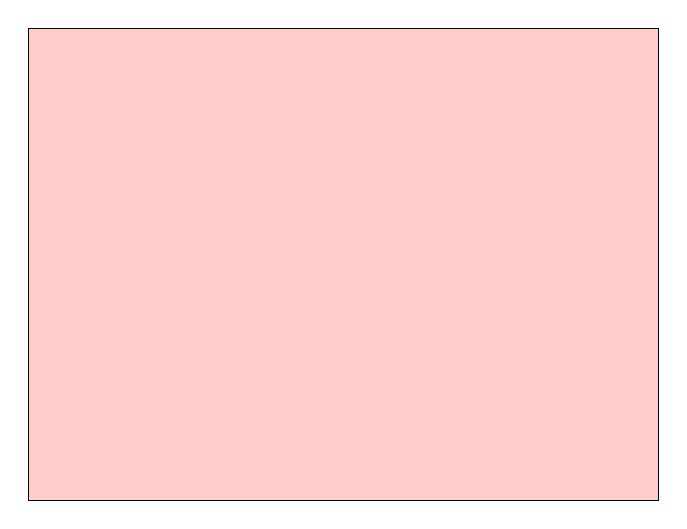
\begin{tikzpicture}[scale=2] 
  \tkzDefPoint(0,0){O}
  \tkzDefPoint(2,-1){A}
  \tkzDefPoint(1,1){B} 
  \tkzDrawSector[color=bistre,dashed](O,A)(B)
  \tkzDrawSector[color=Maroon](O,B)(A)
  \tkzDrawPoints(A,B,O)
  \tkzClipSector(O,B)(A)
\draw[fill=red!20] (-1,0) rectangle (3,3);
\end{tikzpicture} 
\end{tkzexample}
\end{center}
 

 
  \endinput  
  
